%\documentclass[10pt,a4j]{utjarticle}
\documentclass[b5j,twoside,twocolumn]{utarticle}
%\documentclass[b5j,twoside]{utarticle}
%\documentclass[b5j,twoside,twocolumn]{utbook}
\setlength{\columnsep}{2zw}
\usepackage{bxpapersize}
\usepackage{pxrubrica}
\rubysetup{<hj>}
\usepackage{endnotes}
\usepackage{multicol}
\usepackage{plext}
\renewcommand{\theendnote}{[後注\arabic{endnote}]}
\renewcommand{\thefootnote}{\arabic{footnote}}
\usepackage{pxftnright}
\usepackage{fancyhdr}
\setlength{\topmargin}{5mm} % ページ上部余白の設定(182mm x 257mmから計算)。
\addtolength{\topmargin}{-1in} % 初期設定の1インチ分を引いておく。
\setlength{\oddsidemargin}{21mm} % 同、奇数ページ左。
\addtolength{\oddsidemargin}{-1in}
\setlength{\evensidemargin}{17mm} % 同、偶数ページ左。
\addtolength{\evensidemargin}{-1in}
\setlength{\footskip}{-5mm}
%\setlength{\marginparwidth}{23mm}
%\setlength{\marginparsep}{5mm}
\setlength{\textwidth}{225mm} % 文書領域の幅(上下)。縦書と横書でパラメータ(width / height)の向きが変わる。
%\setlength{\textheight}{150mm} % 文書領域の幅(左右)
\makeatletter
\def\@cite#1#2{\rensuji{[{#1\if@tempswa , #2\fi}]}}%%
\def\@biblabel#1{\rensuji{[#1]}}%%%
\makeatother
\usepackage{enumerate}
\usepackage{braket}
\usepackage{url}
\usepackage[dvipdfmx]{graphicx}
\usepackage{float}
\usepackage{amsmath,amssymb}
\newcommand{\relmiddle}[1]{\mathrel{}\middle#1\mathrel{}}
\usepackage{ascmac}
\usepackage{okumacro}
\usepackage{marginnote}
%\usepackage[top=15truemm,bottom=15truemm,left=20truemm,right=20truemm]{geometry}
\usepackage{cleveref}
\usepackage{plext}
\usepackage{pxrubrica}
\usepackage{amsmath}
\usepackage{fancybox}
\usepackage[dvipdfmx]{graphicx}
\usepackage{cancel}
\setcounter{tocdepth}{3}

%\renewcommand{\labelenumi}{(\Alph{enumi})}
\usepackage {scalefnt}
\makeatletter
\@definecounter{yakuchu}
\@addtoreset{yakuchu}{document}% <--- depende on class file
\def\yakuchu{%
\@ifnextchar[\@xfootnote %]
{\stepcounter{yakuchu}%
\protected@xdef\@thefnmark{\theyakuchu}%
\@footnotemark\@footnotetext}}
\def\yakuchutext{%
\@ifnextchar [\@xfootnotenext %]
{\protected@xdef\@thefnmark{\theyakuchu}%
\@footnotetext}}
\def\yakuchumark{%
\@ifnextchar[\@xfootnotemark %]
{\stepcounter{yakuchu}%
\protected@xdef\@thefnmark{\theyakuchu}%
\@footnotemark}}
\makeatother

\usepackage{atbegshi,etoolbox}

\newcounter{newfoot}
\patchcmd{\footnotetext}{\thempfn}{\thenewfoot}{}{}

\newcommand{\evenfootnote}[1]{%
  \ifodd\value{page}%
    \footnotemark%
    \AtBeginShipoutNext{%
      \stepcounter{newfoot}\footnotetext{#1}%
    }%
  \else%
    \stepcounter{newfoot}\footnote{#1}%
  \fi%
}


%\makeatletter
%¥def¥section{¥@startsection {section}{1}{¥z@}{-2.5ex plus -1ex minus -.2ex}{2.5 ex plus .2ex}{¥Large¥bf}}
%\def\mysubsection{\@startsection {subsection}{1}{\z@}{-1.5ex plus -1ex minus -.2ex}{2.3 ex plus .2ex}{\large\bf}}
%\def\subsubsection{\@startsection {subsubsection}{1}{\z@}{-2.5ex plus -1ex minus -.2ex}{.3 ex plus .2ex}{\large \bf $\spadesuit$ }}
%\makeatother

\newcommand{\mysection}[1]{\vspace{-5mm}\section{#1}\vspace{-2mm}}
\newcommand{\mysubsection}[1]{\vspace{-6mm}\subsection{#1}\vspace{-2mm}}


\pagestyle{fancy}

\title{\tbaselineshift =4.0pt クリスチャン・ボルタンスキーと「亡霊」------哲学への架橋のために}
\author{武澤里映}
\date{\vspace{-5mm}}
\setcounter{page}{60}

\begin{document}
\maketitle

\setlength{\footskip}{-2mm}
\lhead[]{【論考】}
\chead[]{}
\rhead[クリスチャン・ボルタンスキーと「亡霊」------哲学への架橋のために]{}
\lfoot[]{\thepage{}}
\cfoot[]{}
\rfoot[\thepage{}]{}

\let\yakuchu=\endnote
\renewcommand{\footnoterule}{\noindent\rule{100mm}{0.3mm}\vskip2mm}
%\tableofcontents
\thispagestyle{fancy}
\section*{序}

作品名は《》、作品のシリーズ名は「」を使用した。個々の作品名については『クリスチャン・ボルタンスキー Lifetime』展図録(二〇一九年)に則っている。
\setcounter{section}{0}
\mysection{はじめに}
クリスチャン・ボルタンスキー(一九四四〜)は、記憶や死、存在と不在などをテーマにした作品を発表している現代アーティストである。子供たちの顔が引き延ばされて額に入れられ、祭壇のように展示される「モニュメント」シリーズや、古着を大量に積み上げたり壁面一面に垂らしたりする《保存室(カナダ)》などの作品が有名である。一般的に、ボルタンスキーの作品群は、個別と普遍、生と死、存在と不在という三つの二項対立のそれぞれに則って考察される場合が多い。本稿では、そのようなボルタンスキーの作品に通底する二項対立を、「亡霊」という観点によって包括し見ていくことで、ボルタンスキーの作品のもつ哲学的射程を考証する。


ボルタンスキーにとってのアートとは、以下のように本人が語っている。
\begin{quote}
僕はアートは死を妨げようとする試み、時間から逃れようとする試みだと思っている[中略]そしてその行為の素晴らしい点は、彼が初めからどうやったってやり損なうということを知っていること。アートは常にある種の失敗で、決して勝つことのできない闘いだ。\footnote{クリスチャン・ボルタンスキー+カトリーヌ・グルニエ『クリスチャン・ボルタンスキーの可能な人生』、二〇一〇年、九二頁。(以下、同書を『人生』と略す。)}
\end{quote}


決して理解できず解決できない難問に対して、闘い続けることがボルタンスキーにとっての芸術である。どうしても失敗する試みを、ボルタンスキーは一貫して行い続けている。本稿ではボルタンスキーのすべての作品を扱うことはかなわないが、ボルタンスキーの作品を「亡霊」という観点から解釈していく。現代思想においても「亡霊」という言葉は、ジャック・デリダの『マルクスの亡霊たち』に代表されるように重要な単語の一つである。「亡霊」を感じる時というのは、実在する何物かがいないのにもかかわらず、誰かの気配を感じる時である。そしてしばしばその「亡霊」という存在は、その名の通り、この世からすでに実体を失った死者と関連付けられ、死んでいるはずなのに現れる何物かとして理解される。つまり、「亡霊」とは、死んでもいなく、生きてもいない、そして存在していないが、不在でもないものと定義づけられる。時間と死に抗い続けるボルタンスキーの作品には、「亡霊」と言いうるような二項対立の狭間にいる何者かが見え隠れしている。本稿ではボルタンスキーの作品と哲学の連結への準備段階として、ボルタンスキーの言葉を中心に分析しながら、個別と普遍、生と死、存在と不在という三つの二項対立の中にまみえる「亡霊」という観点から作品を整理していく。これはまた、一般的な芸術作品の鑑賞とは全く違う感覚をもたらすボルタンスキーの作品への、新たな芸術の可能性を示唆するための試みでもある。


まず第1章では、ボルタンスキーにとって最重要である特殊性から普遍性への移行について、初期作品の「復元」シリーズやその後の「モニュメント」シリーズを手がかりに記述する。そこには、決して全体的なものへとは回収されない個別の主体でありながら、普遍性をもち鑑賞者によって作り出される「亡霊」がいることが示唆されるだろう。次に第2章では、ボルタンスキーが時間と同様に芸術が抗うものとしてきた死について、再び初期作品から「モニュメント」シリーズ、《保存室(プーリム祭)》、《死んだスイス人の資料》、古着を用いた《保存室(カナダ)》といった、生と死にまつわる作品を分析しながら、死んでいながらも生きている「亡霊」をみる。そして最後に、「存在と不在」というボルタンスキー最大のテーマに則って、ボルタンスキー自身が自らの死を自覚し始めた二〇〇〇年代以降の作品に着目し、ボルタンスキーが「亡霊」となりうる道程について解釈を試みる。


\mysection{個人と全体の間で}
ボルタンスキーにとっての最大の関心は、「最も個人的なものから最も総体的なものへの移行」\footnote{『人生』、八九頁。}だという。ボルタンスキーは、その作品を通して、死や記憶といった普遍的な問題を、個人の次元にとどまりながら表現することにこだわり続けてきた。個人と集団の媒介として機能するのが彼にとってのアーティストの役割であり、ボルタンスキーは初期作品から一貫して、一般的で無味乾燥な情報にはならない方法で、個人が全体になり普遍性をもつにいたる道程を表現する。
\mysubsection{失敗から立ち昇る普遍性}
ボルタンスキーがアーティストとしての自覚をもって制作した最初の作品であり今まで続く活動に繋がる作品は、一九六九年に作られた小冊子『一九四四年から一九五〇年の私の幼年時代の残存物すべてについての調査と提示』であるが、そこにボルタンスキーは、「死は恥ずかしいことだ。すべてを保存することを試みなければならない。どうやって小さな記憶を救うか…」\footnote{『人生』、五二頁。}と書いた。ここにみるすべてを保存する試みは、その後の「復元」シリーズや《目録》につながっている。それらの作品の、幼少期に使った事物を復元する試みや、誰かが所有している物をすべて展示する試みで考えられていたのは、展示品それ自体は持ち主の人間について何も語らず、むしろ「それを見る人間一人一人が、そこに自分自身のポートレートを見出す」\footnote{『人生』、八四頁。}ということだった。つまり事物を見る側からすれば、そこに見ることができるのはその持ち主の個別性ではなく、それらの事物が自分の人生にも関わり深い身近なものであるが故の、自己の投影なのである。そこでは持ち主の個別性は鑑賞者の個別性に回収され、その鑑賞者の体験が連なることにより個別性が普遍性へ至る。作品を見る人たちそれぞれに抱かれる「亡霊」は自己の投影を踏まえた唯一の物でありながら、それ自体は他の鑑賞者の中にも同様に生まれることで普遍性をもつ。「復元」シリーズや《目録》といった同じ作品を見る鑑賞者は、身近な事物にまとわりつく自分自身をそこに見る。しかし、この試みは、鑑賞者のうちの特定の能力や知識をもった限定された人だけではなく、すべての鑑賞者が可能な試みなのである。ここにおいて、個人の自己が投影されるという意味で個別的でありながら、誰にでも存在しうる普遍的な「亡霊」がいることが分かる。


ボルタンスキーの写真を用いた作品も、上記のような性質をもつ。一九七二年の、ボルタンスキーにとって写真アルバムを用いた最初の作品である《D家の写真アルバム》は、ボルタンスキーの親しい友人だったシャルル・デュランの家族写真を用い作られた。ボルタンスキーはこの写真を用いた理由に、デュランという名前やその家族写真がフランス中流家庭の典型的なものだったことを挙げている。この作品の制作中、ボルタンスキーは「家族写真というのは決して現実を写すものではなくて、皆が固定観念としてもっている「模範的」家族のイメージを反映するものだ」\footnote{『人生』、一一〇頁。}という考えを得た。さらに同年の『一九四六年から一九六四年のクリスチャン・ボルタンスキーの十枚の肖像写真』でもまた同様の、社会に浸透する固定観念を見せる取り組みが行われている。このアルバムは、一見するとボルタンスキーの様々な年齢の写真が収められ、年齢別にキャプションがふられた写真がつづられているように思われるが、よく見ると背景の一致や被写体の動作などが不自然な写真が多い。つまり、これはボルタンスキーの成長アルバムなどではなく、様々な個人をボルタンスキーに見立てた、演出された作品なのである。ボルタンスキーはこの作品についてこう語っている。
\begin{quote}
僕が言いたかったのは、「クリスチャン・ボルタンスキー」というのは一人の特定の人間ではなく、あらゆる子供たちであり得るということだった。僕がイニシャルの「C.B.」をよく使っていたのも同じ理由で、その方がより包括的で、一般的子供時代を反映できると思ったからだ。\footnote{『人生』、八九頁。}
\end{quote}


ボルタンスキーはここで自身のポートレートを直接的に他者のもつイメージと重ね合わせることを試みている。彼は写真が個別性をもつと同時に、その複製可能性や交換可能性によって普遍的なものになることを示唆する。復元した事物や誰かの所持品と同様に、写真は本来個人を記録し証明するものであるはずが、ボルタンスキーによってそれは他者にも適用可能になってしまうのだ。
\mysubsection{\tbaselineshift =3.0pt 匿名の宗教性------「モニュメント」シリーズを中心に}
「モニュメント」シリーズは、拡大され額に入れられた子供の顔写真が祭壇もしくは墓標のように展示されるインスタレーション作品である。初期作品の段階では、《D家のアルバム》に見られるような「典型的なフランス人」などといった社会のなかに浸透したイメージだったものが、この「モニュメント」シリーズにおいて、より広範な対象が受容可能な宗教性に推移していく。「モニュメント」シリーズは、ボルタンスキーが個人の代わりのきかないかけがえのなさに関心を持つことで生まれた。その意味で、初期作品と同様に、個別の鑑賞者は写真のそれぞれに自己投影を試みることができる。しかしまた、これらの作品には特定されえない宗教性があふれている。ボルタンスキーはこれらに意図的に、何か特定の宗教を示唆するものではなく、個人が生活の中で見たことがあるお寺や教会などを総合したような、普遍的な宗教性を与えている。「モニュメント」シリーズで示唆される宗教は、あくまで宗教性であり、特定のものではない。つまり、それは初期作品にも通じるような、一般的な通念としての宗教なのである。初期作品と違うのは、それらはもはや実際の社会などの共同体に妨げられることがないという点である。


一方これらの作品で作られる祭壇は、普遍的な宗教性をイメージさせながらも、それらは大理石などの素材ではなく、取るに足りない素材で神聖さが演出されている。そこには絶対的な力ではなく、人間的な弱さ、貧しさが表現されている。失われていくものをいかにとどめられるのかという、解決不可能な困難に対しての自覚的な仮の答えがある。このような人間的な弱さ、貧しさは、ボルタンスキーにとってあくまで作品が個人的な次元にとどまるために必要なものである。ボルタンスキーは自らの作品にある種の遊び心を取り入れる。それらは整った美をもつわけではなく、あくまでも作品は完璧ではないのだ。ボルタンスキーの作品は、均整のとれた静謐で完全な作品を目指さない。完全な答えが準備されていることは、ボルタンスキーにとっては悪いことなのである。\footnote{ボルタンスキーは彼にとっての悪い宗教と好ましい宗教の違いについてこのように語っている。
「この世界には二種類の宗教が存在すると思います。一つは、人々が答えを持っていると信じている宗教で、それは私にとっては悪い宗教なのです。もう一つは、答えはないけれども、問いを投げかけ、個々の問いの後にまた新たな問いがやって来ると信じている宗教です。しかし、続くのは問いのみです。答えを持たずに問いを繰り返す宗教のほうが、答えを持っている人々よりもずっと好ましいと感じます。」以下の二〇一八年に行われた対談を参照。クリスチャン・ボルタンスキー、杉本博司『クリスチャン・ボルタンスキー Lifetime』展図録、二〇一九年、一〇五頁。}そして、ボルタンスキーは、キリスト教に対しそのヒューマニズムを認める意味でこのように言う。
\begin{quote}
神としてのキリストよりも一人の人間としてのキリストが好きなんだ。僕は、間違ってるか当たってるかは別として、このことをちょっと複雑に考えてみた。つまり、これは神に対する人間の闘いで、キリスト教の偉大さはこの勝利=敗北の中に、少なくとも神に対する人間の反逆の中にあるということ。[中略]キリスト教の中にはある種のヒューマニズム、個としての人間を重要視する気持ちがあると思う。\footnote{『人生』、一五〇頁。}
\end{quote}


ボルタンスキーはキリスト教を肯定しているが、いわゆる「神」を素直に肯定しているわけではない。そして同時に、神を否定しているわけでもない。彼にとって神とは時間であり、生と死を支配する存在である。そうした神、つまり時間に立ち向かう行為をボルタンスキーは人間らしい営みとする。


ボルタンスキーはまた、名前を与えることを重要視する。《死んだスイス人の資料》などのシリーズでは、膨大な量の名前が使われる。名前を与えることはすなわちその人間の唯一性を認めることであり、これにより個人は集団より分離する。ボルタンスキーの作品が抽象化され一般的な情報へと回収されないために、そして作品が個人の次元にとどまり続けるために、名づけは必要な措置である。実際に、ボルタンスキーは個人の名前以外にも、作品や展覧会の名前にもこだわりをもち制作を行っている。\footnote{ボルタンスキーは作品の名前について、実際に亡くなったスイス人の写真を用いた作品を例にこう語っている。
「例えば『死んだスイス人』は本当に死んだスイス人だったし、僕は「ラスプーチン」的に、アートを口実にして死とか神聖なものを犯すのは好きじゃない。だからタイトルはとても重要なんだ。もし「死んだスイス人」の代わりに「英国倶楽部のメンバーたち」とかつけたら全く別のものになってしまう。」以下の文献を参照。『人生』、二八一~二八二頁。\\また、同文献中では、タイトルに関して以下のようにも語っている。
「作品や展覧会のタイトルはとても重要視している。最初の展覧会からすべて名前を付けてきたし、いつも二重の意味を持った題を探してきた。」以下の文献を参照。同前、二四八頁。}しかし一方で、名前は簡単にその唯一性を奪われる。ボルタンスキーの初期の作品では、クリスチャン・ボルタンスキーなどといった固有の名前を冠しながらも、被写体は必ずしもボルタンスキーではなかった。個人と名前の乖離を、ボルタンスキーはどのように解消しているのかについては、さらなる考察が必要である。

\mysubsection{まとめ}
 ボルタンスキーは、アーティストとは「事実や虚構を含めて自分自身の話をしながら、実は誰もがその中に自分を確認できるような、あらゆる人間のことを語る存在」\footnote{『人生』、九〇頁。}とする。芸術はそこに新しい何かを発見するものではなく、そこに当てはまる自分がいることを確認できる行為なのだ。そうした自分の確認は、あらゆる個人がそれぞれに行うことで普遍的なものとなる。しかし、確認される自分は、常にそこには存在しないある誰か、つまり「亡霊」に重ね合わされて初めて確認される。ボルタンスキーが世界で最も崇拝するものだとするカントールの演劇について、彼はこう語っている。
\begin{quote}
彼(カントール)の作品はどれも亡霊をめぐるものばかりで、僕たちの記憶の中に充満している様々な亡霊を滑稽に、あるいはグロテスクな形で蘇らせる。でもカントールは天才だから、そこに登場するのは彼個人の亡霊であると同時にポーランドの亡霊でもあって、大きな歴史と小さな歴史が混じり合っているんだ。これはまさに僕がやろうとしていることだ。\footnote{『人生』、九三頁。}(カッコ内筆者による補足。) 
\end{quote}


ボルタンスキーはあらゆる鑑賞者に、特定の誰でもない「亡霊」を見出させていく。鑑賞者はその作品に現れる事物や宗教性が自身の生活にも身近な事物だと気づき、それによって自己を投影しながら、作品にまとわりつく生の気配を何物かに収縮させる。しかし、それは自己を投影しているからといって自分ではないし、かといえば他の誰か特定の人であるというわけでもない。それらは自己投影によってそれぞれの個別性が保たれてながらも、そのような人物像は誰しもが想像することが出来る。「亡霊」は名前をもたない。それは「亡霊」という言葉でのみ示され、それが女であり髪が長く見えたとしても、それが本当に誰であるのかを知る手段はない。しかしそうであるがゆえに、「亡霊」は万人に感じられうる。「亡霊」は、個別性をもちながらも、それによって特定されない。ボルタンスキーが作品を通じ促すのも、個人が自己を投影し生み出す不在の誰かであり、そしてそれは各人が抱く故にもはや個人のものではない。それは塚原が指摘するような、「類としての人間の記憶を呼び起こす」\footnote{塚原史、「ボルタンスキーの暗い箱 またはその重さについて」、一九九〇年、一三七頁。}ことだと言える。

\mysection{生きてもなく、死んでもいない存在として}
ボルタンスキーは自身の試みを「痕跡を残すこと、死と闘うこと」\footnote{『人生』、五二頁。}だとして作品を制作してきた。こうした死とボルタンスキーの関係は、一般には「モニュメント」シリーズや、ユダヤ人に関わる作品の中で特に取り上げられることが多いが、死に対する洞察は彼の作品の中で一貫している。関昭郎が「彼の死に対する興味は、人に対する興味から生まれている」\footnote{関昭郎「ボルタンスキーと死の方便」、東京都庭園美術館編『クリスチャン・ボルタンスキー アニミタス_さざめく亡霊たち』展図録、二〇一七年、一〇四頁。}と分析するように、ボルタンスキーが考える死は、必ず個人との関わりの中に属するものだった。抽象的な死ではなく、一人の個人の死を考え続けているのである。
\mysubsection{子供時代の自分という「亡霊」}
一九六九年に作られた小冊子『一九四四年から一九五〇年の私の幼年時代の残存物すべてについての調査と提示』の中で、ボルタンスキーは失われていくものをどうやって残していくのかという難題に向き合っていた。ボルタンスキーのいう「死を妨げようとする試み」が始まったのである。そのようなボルタンスキーの作家人生は、その後《クリスチャン・ボルタンスキーの日用品を入れた日付付きのビスケット缶》や《一九五一年にクリスチャン・ボルタンスキーが所有していた一組の長靴の粘土による復元の試み》などの超個人的な作品を主にして始まる。しかし、彼は早々に復元の不可能性に気づいてしまう。復元した事物は過去のボルタンスキーについては何も語らない。ボルタンスキーは、そのような復元できない幼少期の自分について、こう語っている。
\begin{quote}
小さなクリスチャンは死んでしまった、僕はもう彼には似ていないし、同じ考え方もしない。それでも僕は彼のことを知っているし、たとえ死んでしまったとしても、僕の記憶の中に常に存在している。人間にとっての初めての重要な死の体験は子供時代の死だ。\footnote{『人生』、九二頁。}
\end{quote}


ここで重要なのは、ボルタンスキーは過去の自分を今の自分と連続したものではなく、分断されたものとして考えているということである。ここで、彼自身の中にとどまり続けながらも死んでいる最も身近な「亡霊」としての幼少期を考えることができる。


そのような「失敗」としての「復元」シリーズは、その後の普通の人の所有物をすべて展示する作品《目録》につながる。この《目録》は、「復元」シリーズと同様に一九六九年の小冊子のアイディアを出発点とし、「一人の人間があとに残したものを全部集めて、虚ろなポートレートを浮かび上がらせること」\footnote{『人生』、八三頁。}が目指されていた。そのような目録は、第1章で見たような鑑賞者によるポートレートという考えに加え、「保存しようとするものは全て死んでいく」、つまり「一つのイメージを固定させようとするのは、死に繋がる行為だ」\footnote{どちらも『人生』、八四頁。}という概念を下敷きにしていた。生き生きとしたものは、保存するために取り上げることによって死んでしまう。保存のためのパラドキシカルな構図の中に、ボルタンスキーは死を見ている。


このような「目録」シリーズの原型は、一九七二年の《フランソワ・Gの衣類》とされる。これは一人の子供の衣類をすべて展示した作品であり、この作品には「僕たちは皆内面に死んでしまった子供を秘めている、そして歳を取るにつれてこの失われた子供を忘れてしまう」\footnote{『人生』、八八頁。}という考えが基礎にあった。こうした手法によって作られた作品は、ボルタンスキー自身が「失ってしまった過去自身を取り戻すために、子供に訴えかけていた」\footnote{『人生』、八九頁。}と話すように、ボルタンスキー自身にとっても、失ったものを取り戻す復元の試みだった。しかし、「目録」シリーズにおいて、このような復元の試みそれ自体が対象を切り離し殺すことだと自覚されるのである。

\mysubsection{\tbaselineshift =4.0pt 写真と死---被写体の生}
その後、ボルタンスキーは一九七二年の《D家のアルバム》を機に、写真を自身の作品に取り入れていく。写真は一般的には事物を保存するために撮影されるものであるが、彼にとってはここでもまた死が絡み合うことになる。一九七五年にボルタンスキーは《ベルリンの子供たち》という写真作品を作る際、子供たちの撮影にて、写真の暴力性にさらされることとなる。

\begin{quote}
写真を撮りながら、[中略]僕は突然子供たちを殺しているような気持になったんだ。並んで待っている子供たちは、まるで銃殺されるのを待っているかのようだった……こんな風に一列に並んでいる子供たちを前にして、それに僕が言葉ができないから何も話しかけられなかったという状況もあって、ある人間を写真に撮るというのは、その人を殺すことだという印象を強く受けてしまった。\footnote{『人生』、一一六頁。}
\end{quote}


このような写真による死は、「目録」シリーズに関しても語られた、何かを保存するための死だということができるだろう。ボルタンスキーはこの経験によって、死のみならず、それを生み出してしまえる写真を撮るという行為それ自体への恐怖もまた感じたのではないだろうか。


そのような死と写真の関係が明確に作品化されたのが、「モニュメント」シリーズだろう。一九八五年からつくられたこのシリーズは、ボルタンスキーがその直前に作っていた「コンポジション」シリーズから脱し、初期作品へと立ち返り作られたものである。この時期からボルタンスキーは意図的に宗教性を取り入れる。制作の中、繰り返されていた意識は、以下のようなものだった。
\begin{quote}
ニキビ面のとるに足らないこの子供たちは、僕にとってはみんな聖人だ。でも聖人であると同時に死者でもあるんだ。なぜならこのイメージは十年以上も前のもので、今ではもう違う存在になってしまっているだろうから。\footnote{『人生』、一四八頁。}
\end{quote}


もはや写真に写ったのと同じ人物はいない現実の中、ボルタンスキーはその状況を成長ではなく死ととらえる。「モニュメント」シリーズに掲げられた子供の写真は、もちろん鑑賞者を写していない。しかし、こうして掲げられた写真を見る時、その被写体の子供たちは他人のようには思えない。不気味な既視感の理由は、鑑賞者自身もまた繰り返し殺してきた過去の子供の自分を投影することにある。子供を写真に撮るような普通の行いとして、大人は常に自分の中の子供を殺すのだ。その制作の体験は、ボルタンスキーにとって、「幽霊を相手に作品を作っているよう」\footnote{『人生』、一四八頁。}だったという。

\mysubsection{時への対抗としての生き返り}
ユダヤ人の写真を用いた作品と同時代に作られた《保存室(カナダ)》などの古着を用いた作品は、大量の古着が積み重ねられ、圧倒的な数とともに、着用者の不在に注意を向けさせる。このような衣服の利用は写真と連なるものであり、「無名の人々の写真や衣服はすべて、存在/不在を表現していて、誰かがいる、誰かが生きていた、ということなのである」\footnote{『人生』、二三〇頁。}と語られる。この作品において、古着の着用者はそれぞれ不在であり、写真作品でのボルタンスキーの考え方を適用するならば、古着は機能を剥奪され死んでしまっている。しかし、こうした死んでいるものとしての古着にとって特有なのは、それらが再び生き返ることができることだ。一九九四年にサン・トゥスタッシュ教会で行われたインスタレーションにおいては、作品に使われたコートがサラエボ行きのトラックに信者によって積み込まれた。ここでの経験についてボルタンスキーはこのように語っている。

\begin{quote}
僕にとって意義深かったのは、床に並べられていた時には、過去をなくしたいわば死んでしまっていたコートが、サラエボで復活して、再び人々に愛されるようになるということだ。一度は死んでしまったものたちが、僕たちが知ることのできないまた別の生を受けるということ。\footnote{『人生』、一七六頁。}
\end{quote}


死んでいたはずの古着は、また再び機能を持った状態へと戻っていく。これは写真や美術館にも通じる脱文脈化への抵抗であり、ボルタンスキーにとっての保存という難問への新しい答えなのではないかと考えられる。
\mysubsection{まとめ}
ボルタンスキーにとって死とは、単純に心臓が止まることでも、その身がどこかへ失踪することでもない。実体は、存在と不在を扱う作家にとって問題ではなく、むしろ過去の自分と同じであり続けられるのかということが問題なのだ。死とは、何か特別なことでもなく非日常のことでもなく、常に人が隣接している領域のことである。特定の誰かが死ぬということは、特定の誰かによってのみ完遂されるという点、そしてそれがまったく特別なものでもなく、子供の頃から行い続けてきた行為であるという点で、ボルタンスキーの考える死は、第1章でみたような個人と普遍にまたがっていく構造をもっている。そしてさらに、そこで死んだとされる何者かは、私たちの中に想起の形で存在している。ボルタンスキーにとって死は完全な終わりではない。むしろ、死んだ後に忘れ去られてしまうことが終わりであり、彼が作品によって抗おうとすることである。「亡霊」もまた、死んでいるはずの人間が、個人が見ている世界の中に現れることで生きていく。それは見ている人の内部でのみ存在し、他の人に同じ「亡霊」が見えているかどうかを確かめるすべはない。しかし、眼前にいる限り、「亡霊」は生きているのだ。ボルタンスキーの作品を通じ抱かれるのも、すでに死んでいるはずのものが想起により蘇るという経験である。それはまさしく「亡霊」を見る経験だろう。

\mysection{\tbaselineshift =3.0pt 存在と不在の間------物語としての作品}
一九八六年に行われた「暗闇のレッスン」展は、ボルタンスキーにとって「空間のアーティスト」となる転換点だった。正確な時期は不明だが、このころからボルタンスキーは自分の展覧会の中に、「進展と逆転を含んだ時間の概念を取り入れようとしてきた」\footnote{『人生』、二七四頁。}と推察される。初期の短編映画作品も物語性を多分に含んではいるが、だいたい二〇〇〇年以降から、ボルタンスキーは物語の主題を取り上げるようになる。「おとぎ話」、「神話」、「物語」などの言葉で語られる作品は、消滅や時間などの主題を扱い、もはや人の域を超えて、「亡霊」さえいない場へと変化しているようにも感じられる。しかし、そこに「亡霊」は本当にいないのか。


このような作品に至る変化は、ボルタンスキーの死に対する感情の変化に付随していると推測できる。ボルタンスキーはここ二十年ほどで、自身の死を暗示させるような展覧会などを複数行っており、作品の中にも自己の死というテーマが現れるようになっている。芸術を「死を妨げようとする試み」とした作家は、自らの死に向き合い、死を受け入れ始めているのだ。ボルタンスキーはこのような自身の死を近くに感じている瞬間を、人生に三回訪れた「創造的瞬間」のひとつだといい、この折に、「アートにもっとも近づいた」と感じるのだと語る。\footnote{ボルタンスキーは自身の作品の転機について以下のように語っている。
「自分の人生で三回の創造的瞬間がありました。最初は七二年頃で、大人へと成長した時期。[中略]二回目は八二年、八九年の両親の死です。[中略]それから最後は数年前から、刹那的な作品や、旅を中心とした制作に取り組んでいます。大人になったとき、両親との別れ、そして死が近づいてきたとき。こういった節目の折が、アートにもっとも近づいたと感じる瞬間なのです。」以下の文献を参照。クリスチャン・ボルタンスキー、三木あき子「ARTIST INTERVIEW CHRISTIAN BOLTANSKI クリスチャン・ボルタンスキー」『美術手帖』六八(一〇四六)、二〇一六年、一九九頁。}

\mysubsection{\tbaselineshift =3.0pt 自覚的な崩壊------近年のインスタレーションの傾向から}
近年ボルタンスキーが手掛ける作品は、徐々にその消滅を特徴とするものが多くなっている。その土地や建物、展覧会場のサイト・スペシフィック性を利用したインスタレーションや、《心臓音のアーカイブ》、「アニミタス」シリーズ、《ミステリオス》などがその典型である。前者のようなインスタレーションは、展覧会が終われば取り壊される。作品は物体ではなく、ボルタンスキーからの指示書によって成立する。ボルタンスキーはこのような作品の形態を楽譜になぞらえ、再解釈されることを望んでいる。あれほど時による記憶の忘却に抗い続ける作品を作っていたボルタンスキーはどのように変わったのだろうか。このような仮設性の強い作品について、ボルタンスキーはこのように語る。

\begin{quote}
僕のパラドックスは、伝達とか形象とかいう問題をあれこれ考えて、作品も墓碑のようなものばかりなのに、現実にはどんどん壊す傾向が強くなって、残るのはアイディアだけという点だ。\footnote{『人生』、二五二頁。}
\end{quote}


これ以前の時期のボルタンスキーの作品は、常に抗いきれないものに対する闘いであった。それらは、写真や古着などを用いて、不在や記憶の不可能性を直接表現していた。しかしここにおいて、ボルタンスキーは事物による表現から離れている。残すためのものを作りながら、それらを壊していく。一見矛盾しているように見えるこの志向は、ボルタンスキーによるとこのように説明される。


\begin{quote}
僕の仕事に常につきまとっているもので、生き延びたいという願望、「永久に」というテーマに関わりながら、でも同時にこの「永久」は消滅ぎりぎりのところにあって、そして最後には消えていく…。\footnote{『人生』、二五五頁。}
%\begin{quote}
\end{quote}


この境地に至るまで、常に彼は失敗の当事者だった。そうした失敗は、成功を目指しながらも否応なく導かれてしまうものだった。しかし、ここにおいて、復元や記録の試みに失敗していた彼は、自覚的に失敗やその崩壊を見据えている。

\mysubsection{実在することに意味はない\tbaselineshift =3.0pt------「神話」としての作品}
一方で、《心臓音のアーカイブ》、「アニミタス」シリーズ、《ミステリオス》などの作品は、インスタレーションと同様に、仮設性が強い。これらは、豊島やチリのアカタマ砂漠、カナダ北部やパタゴニアなど、地理的に遠く簡単にたどり着けない場所に置かれた作品を、鑑賞者は展覧会場で映像などによって間接的に鑑賞する。ボルタンスキーによると「おとぎ話」だと言われるこのような作品は、世界に確実に存在していながらも、それを確かめに行くことは簡単ではない。さらにこれらの実際の作品は、簡単に壊れてなくなる。ボルタンスキーはこのような作品の在り方について、こう語っている。
\begin{quote}
その物語は存在し続ける。私の名前が消えても、その場所は巡礼場所のように残る。作品が実際にあるかどうかは、本当はそれほど重要ではなくて、その神話が存在する、ということが大事なのです。\footnote{以下の文献中の二〇一六年に行われたインタビューから引用した。
クリスチャン・ボルタンスキー、関口涼子「クリスチャン・ボルタンスキー インタビュー」東京都庭園美術館編『クリスチャン・ボルタンスキー アニミタス_さざめく亡霊たち』展図録、二〇一七年、四九頁。}
\end{quote}


作品が実在し、自身の目の前にあることは問題ではない。ボルタンスキーやその作品が消えようと、物語を知る人が一人でも存在し、語り継がれることが重要なのである。彼はそうした自身の作品が彼の死後も残ることではなく、一つの物語として伝播されていくことを望む。彼はここで、復元の試み、つまり時と抗う行為を、他者にゆだねるのである。孤独な闘いだった復元の試みは、ボルタンスキーを起点にしたネットワークへと発展するのだ。それは物語の始まりとしての作品だ。

\mysubsection{まとめ}
こうした試みの中で、「亡霊」となるのは誰なのか。ボルタンスキーにとって表現する内容は初期から大きく変わってはいない。しかし、これらの作品には、今までの作品で直接的に提示されてきた、そこに不在する誰かという意味での「亡霊」はいない。ここで、ボルタンスキーが自身がいなくなった後について語っているところに着目したい。ボルタンスキーは作品が残っていく理想のあり方として、自分が設置した作品が残ること、他の人が自分の作品を再解釈し展示すること、そしてボルタンスキーについて後に語られる物語としての「模範的人生」を作成することという3つの方法を挙げる。\footnote{『人生』、二四七~二四八頁。}ここで興味深いのは、最後の「模範的人生」という物語を作ることが、《D家のアルバム》などに典型的な、後から付け加えられる個人性、つまり普遍性を目指しているということである。ボルタンスキーは、自身が亡き後、「かつてクリスチャン・ボルタンスキーという人間がいて、作品は残ってないけど、いろいろな問いを投げかけた人間、物語を語っていた人間がいたという話」が語られていくことを望んでいる。\footnote{『人生』、三〇八頁。}しかし、そのような物語はボルタンスキーでなくとも当てはめられるものでもあるのだ。ボルタンスキーという固有名に付加される話は、それ自体ボルタンスキー以外の人にも当てはめうる話でなければならない。ボルタンスキーが不在の状態で、ボルタンスキーがやったことが伝承されるとき、だれが行ったか確証はない。ここにおいて、ボルタンスキーの「模範的人生」は、個人的でありながら普遍的であり、死んだはずの人間の物語は、語られることによって生きかえる。この神話という物語をめぐって、ボルタンスキーは「亡霊」となることが確約されているのではないか。


\mysection{おわりに}
初期の超個人的な記憶の復元から始まり、宗教性やホロコーストを超え神話に至るボルタンスキーの作品は、表現のみに着目するととらえどころがないかもしれない。しかし、それらはその意味するものによって貫かれていた。ボルタンスキーの作品は、ミニマリズムや芸術の自律性などといった従来の芸術理論や用語によってはすべてを語ることができず、既存の美術史の中でも特異な位置を占めてきた。本稿でボルタンスキーの作品に深く影を落とす「亡霊」を考察することで、ボルタンスキーの作品の新たな位置づけを捜索すると同時に、哲学と芸術の新たな臨界点が提示されただろう。ボルタンスキーの挑む、個別と普遍、生と死、存在と不在という三つの二項対立は、芸術におさまらず、哲学そして人間にとって難問だ。


このような作品からあふれ出る何かについて、小林康夫は重要な指摘を行っており、ボルタンスキーの手掛ける空間について以下のように言っている。少々長いが引用する。

\begin{quote}
この空間の全体が、眼差しをもち、声をもち、そうしてわたしに、「あなたもわたしと同じように人間であるのよ」と告げている。すなわち、生きられた時間を分有することができないのに、(そして時間を分有することこそ、人間の共同体の根源的支えなのに)、にもかかわらず、そうした共同性のはるか手前で、分有できない不可能性そのものを分有するというアポリア的可能性として、絶対的に無名の―ほとんど個別的な「顔」すらまだもっていないような―「人間」があるのではないか。\footnote{小林康夫「クリスチャンにささやく_インファンスの可能な/不可能な儀礼」東京都庭園美術館編『クリスチャン・ボルタンスキー アニミタス_さざめく亡霊たち』展図録、二〇一七年、一七頁。}

\end{quote}


ここでの「人間」は、無名でありながら、実体をもち私たちを見つめる。デリダは、視覚的な現れを強調しながら、亡霊とは、「それによってわたしたちが見つめられている、観察されている、監視されていると感じる誰かのことなのです」\footnote{ジャック・デリダ+ベルナール・スティグレ―ル、『テレビのエコーグラフィー—―デリダ〈哲学〉を語る』、原宏之訳、二〇〇五年、一九二頁。邦訳においては、引用文の主語は幽霊とされているが、湯沢英彦による邦訳も参照し、文脈の都合上亡霊という言葉を主語に用いた。以下の文献を参照。湯沢英彦『死者のモニュメント』、二〇〇四年、二二二頁。}という。ここに、ボルタンスキーの作品との関連を感じずにはいられない。時を超越し現れる「亡霊」は、ここまでで見てきたように、不特定の個人であり、死にながらも誰かの中で生きることを許されている何者かであり、存在と不在を両立している。そして「亡霊」はそうであるがゆえに、人間全体へ通じる可能性をもっているのだ。本稿で見た三つの二項対立は、「亡霊」の中で密接に絡みあう。


最後に、ボルタンスキーが言う「まやかしとしての芸術」について触れたい。ボルタンスキーは「アートの中には「まやかし」があるし、アートは常に虚偽と結びついている」\footnote{『人生』、二八一頁。}と語る。まやかしや虚偽は、ボルタンスキーにとって決して価値の低いものではない。ボルタンスキーはまやかしが見せる普遍性についてこのように語っている。
\begin{quote}
まやかしは真実を見せるものでもあって、嘘を言えば言うほど真実に近づいてしまう。虚偽としてのアートが表現するのは、個人的真実ではなくて一般的真実なんだ。「僕」ではなくて「僕たち」の真実、本質的真実だ。アートの中で最も重要なのは、集団的、普遍的でありながら、一人一人がそこに自分を見いだせる個人的なものでもあること\footnote{同上}。
\end{quote}


個人的なもの、死んでいるもの、存在しないもの、それらが再び普遍性へと移行し、存在し、生き返るためには、「虚偽」のちからが必要だ。このボルタンスキーの言葉は、運命に抗い続ける人間らしい試みとして、想像を頼りにしているように思われる。「亡霊」は私たちの中でこそ生まれる。そしてそこに、「私は、いかなる意味でもペシミストではない」\footnote{塚原史、「ボルタンスキーの暗い箱 またはその重さについて」『美術手帖』(六三一)、一九九〇年、一三六頁。}と語る、ボルタンスキーの深い人間への信頼もまた見えるように思えるのだ。

\clearpage
{\small
\section*{参考文献}
\renewcommand{\labelenumi}{\pbox<y>{[\arabic{enumi}]}}
\begin{enumerate}
\item クリスチャン・ボルタンスキー+カトリーヌ・グルニエ『クリスチャン・ボルタンスキーの可能な人生』、佐藤京子訳、水声社、二〇一〇年。
\item クリスチャン・ボルタンスキー、三木あき子「ARTIST INTERVIEW CHRISTIAN BOLTANSKI クリスチャン・ボルタンスキー」『美術手帖』六八(一〇四六)、二〇一六年、一八五~一九九頁。
\item ジャック・デリダ+ベルナール・スティグレ―ル、『テレビのエコーグラフィー—デリダ〈哲学〉を語る』、原宏之訳、NTT出版、二〇〇五年。
\item 塚原史「ボルタンスキーの暗い箱 またはその重さについて」『美術手帖』(六三一)、一九九〇年、一二三~一三九頁。
\item 湯沢英彦『クリスチャン・ボルタンスキー 死者のモニュメント』、水声社、二〇〇四年。
\item 『クリスチャン・ボルタンスキー Lifetime』展図録(大阪、東京、長崎)、水声社、二〇一九年。
\item 東京都庭園美術館編『クリスチャン・ボルタンスキー アニミタス------さざめく亡霊たち』展図録(東京)、水声社、二〇一七年。
\end{enumerate}
}

\section*{追補}
本稿で扱った作品の制作年代を以下に載せます。諸々(!)の関係で作品画像は準備できず、作品画像が一枚もない作品批評となってしまい申し訳ありません。以下の年表については、クレマン・ディリエによる『クリスチャン・ボルタンスキー Lifetime』展図録中の「クリスチャン・ボルタンスキー年譜」(一八三~一九九頁、小野寺奈津訳)を参照しました。

\begin{table}[ht]
\scalebox{0.78}{
\begin{tabular}{|l|l|}
1944 & ボルタンスキー生まれる。 \\
1969 & 『1944年から1950年の私の幼年時代の残存物すべてについての調査と提示』\\
\raisebox{0.78zw}{1971} & \begin{tabular}{l}
\hspace{-0.55zw}個展「1948年から1954年にクリスチャン・ボルタンスキーが所有\\\hspace{-0.55zw}していたものを復元する試み」を開く。「復元」シリーズが展示される。
\end{tabular}\\
1972 & 《D家のアルバム》\\
 & 《フランソワ・Gの衣服》\\
 & 『1946年から1964年のクリスチャン・ボルタンスキーの10枚の肖像写真』\\
1973 & 「目録」展開催。(カールスルーエ州立美術館)、「目録」シリーズが開始される。\\
1975 & 《ベルリンの子供たち》\\
1985 & 「モニュメント」シリーズの開始。\\
1987 & 《保存室(プーリム祭)》\\
1988 & 《保存室(カナダ)》\\
\scriptsize
1986〜90 & 「暗闇のレッスン」展\\
\footnotesize
90年代以降 & 《死んだスイス人》などのスイス人の写真を用いた作品を多く発表。\\
1994 & サン・トゥスタッシュ教会での古着を用いたインスタレーション\\
2010 & 《心臓音のアーカイブ》\\
2014 & 「アニミタス」シリーズ\\
2017 & 《ミステリオス》\\
\end{tabular}
}
\end{table}



%\begin{figure}[h]
%\begin{tabular}<y>{c}
%\begin{minipage}[c]{0.9\hsize}
 %\begin{center}
  %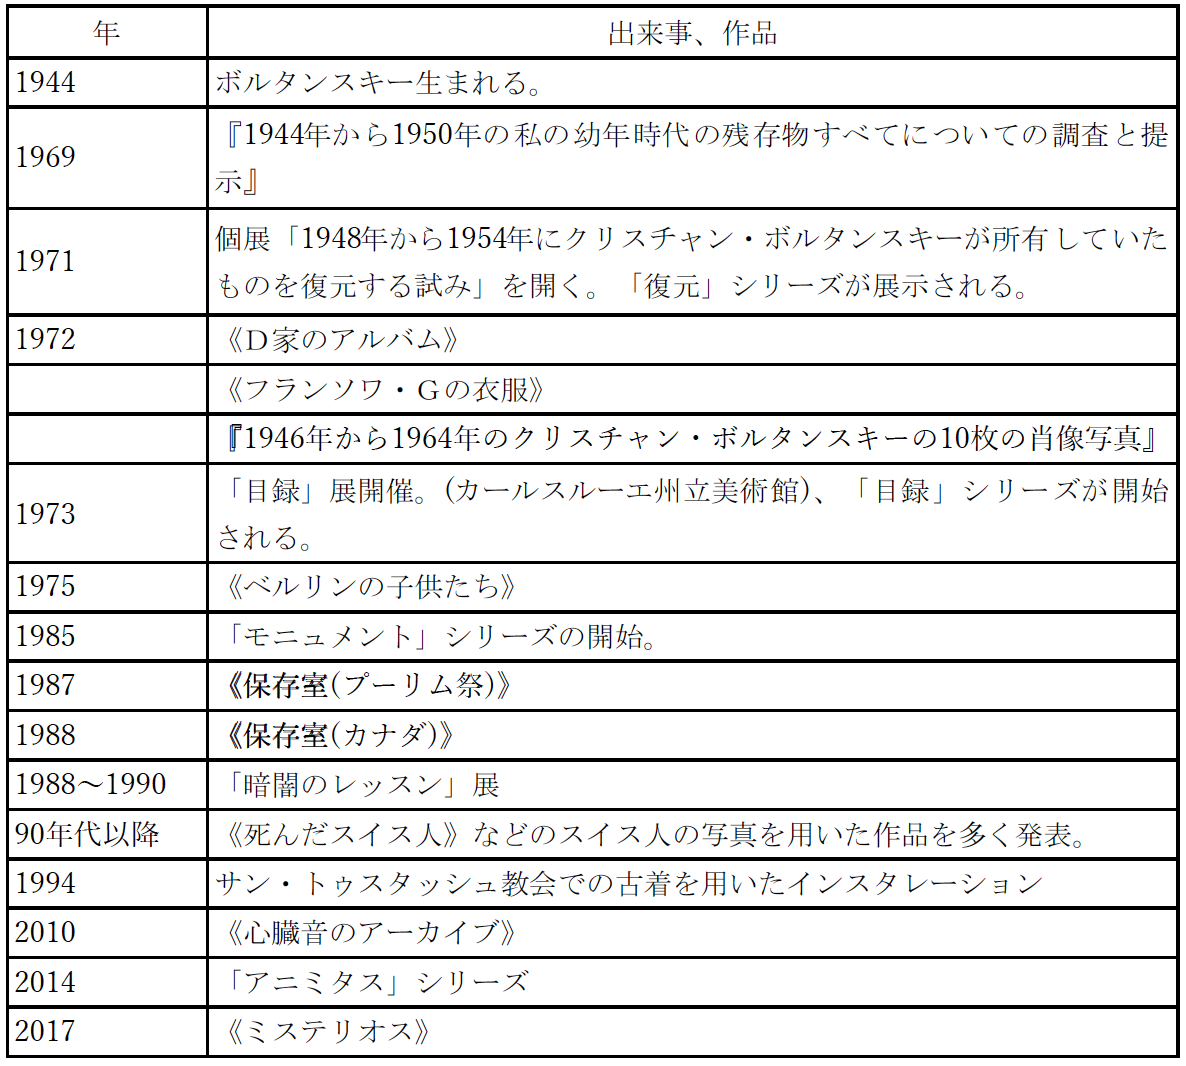
\includegraphics[scale=0.5]{年.png}
  %\end{center}
 %\end{minipage}
%\end{tabular}
%\end{figure}



\end{document}
